\documentclass[thesis.tex]{subfiles}
\begin{document}

\chapter{Prerequisites}\label{chap:basics}
The following sections explain some of the underlying principles that are required to understand the later chapters in this thesis.
Readers that are familiar with the basic concepts of photorealistic and realtime rendering may skip parts of this chapter.

% What belongs here:
% - Mathematics
% - Things that I would expect the reader to know if this would be a paper
% - What constraints are just there
% What does not belong here:
% - References to work that is directly related to the topic

\section{Theoretical Foundation}
This section explains some of the fundamentals of physically based rendering.
For more detailed explanations the reader is referred to the book \emph{Physically Based Rendering, From Theory to Implementation} by Pharr and Humphreys \cite{bib:pbrt}.

\subsection{Physical Foundation}
Light is generally an electromagnetic wave which originates at a light source and is bounced of or absorbed by the surfaces it hits.
As such, there are several complicated physical properties like diffraction,interference and quantization effects (due to the particle properties of electromagnetic waves) which are usually ignored for rendering, as they play most of the time a minor role.
Each light particle (= photon) has a certain wavelength which is responsible for the perceived color.
We are only interested in the visible part of the spectrum which ranges from about $380nm$ to $780nm$.
The number of photons registered by the eye defines the brightness.\\
As the human retina has only three receptors, each with a given range of wavelength-support, it is usually sufficient to perform all calculations using only the three basic color stimuli red, green and blue \cite{bib:colorscience}.
However, as recently pointed out by Meng et al. \cite{bib:spectrumrendering} there are several problems that might lead to color shifts violation of energy conservation. \todo{recheck if I heared that talk (upcoming EGSR)}


\subsection{Radiometric Quantities}
There are several basic quantities that describe the transport and perception of light.


%$\phi$ & \textbf{Radiant Flux}, light power\\
%$I$ & \textbf{Radiant Intensity}, flux density per solid angle\\
%$E$ & \textbf{Irradiance}, flux density per area\\
%$L$ & \textbf{Radiance}, flux density per area per solid angle\\
%$\rho$ & \textbf{Reflectance}, ratio between incoming and outgoing flux\\

L,I,E, the whole zoo

\subsection{Rendering Equation}
Rendering Equation

\subsection{Bidirectional Reflectance Distribution Function}
Introduce theory and Blinn-Phong
separation of Diffuse and Specular

\section{Realtime Rendering}
Super awesome book about EVERYTHING! \cite{bib:RealtimeRenderingBook} (Tomas Akenine-M\"{o}ller and Eric Haines and Natty Hoffman).

\subsection{Local Illumination}


\subsection{Shadow Mapping}
Basics!

\subsection{Deferred Rendering}


\subsection{Deferred Rendering}
Basics only!

\section{Modern GPU Pipeline and Capabilities}
OpenGL 4.5 pipeline picture?
A lot of information about shaders and compute.

\section{Spherical Harmonics}\label{sec:pre:sh}
Spherical Harmonics (SH) are a set of orthonormal basis functions, analogous to the Fourier transform's basis functions, but defined on the surface of a sphere.
They are often used in computer graphics to approximate spherical functions like visibility, lighting or reflectance. Similarly, they will later be used in \autoref{sec:impl:diffuse} to describe the total irradiance for a given normal.

More detailed explanations can be found for example in \cite{bib:grittysph, bib:stupidsph} on which this summary is based.

\subsection{Definition} \label{chap:sh:def}
\begin{figure}[h]
	\centering
	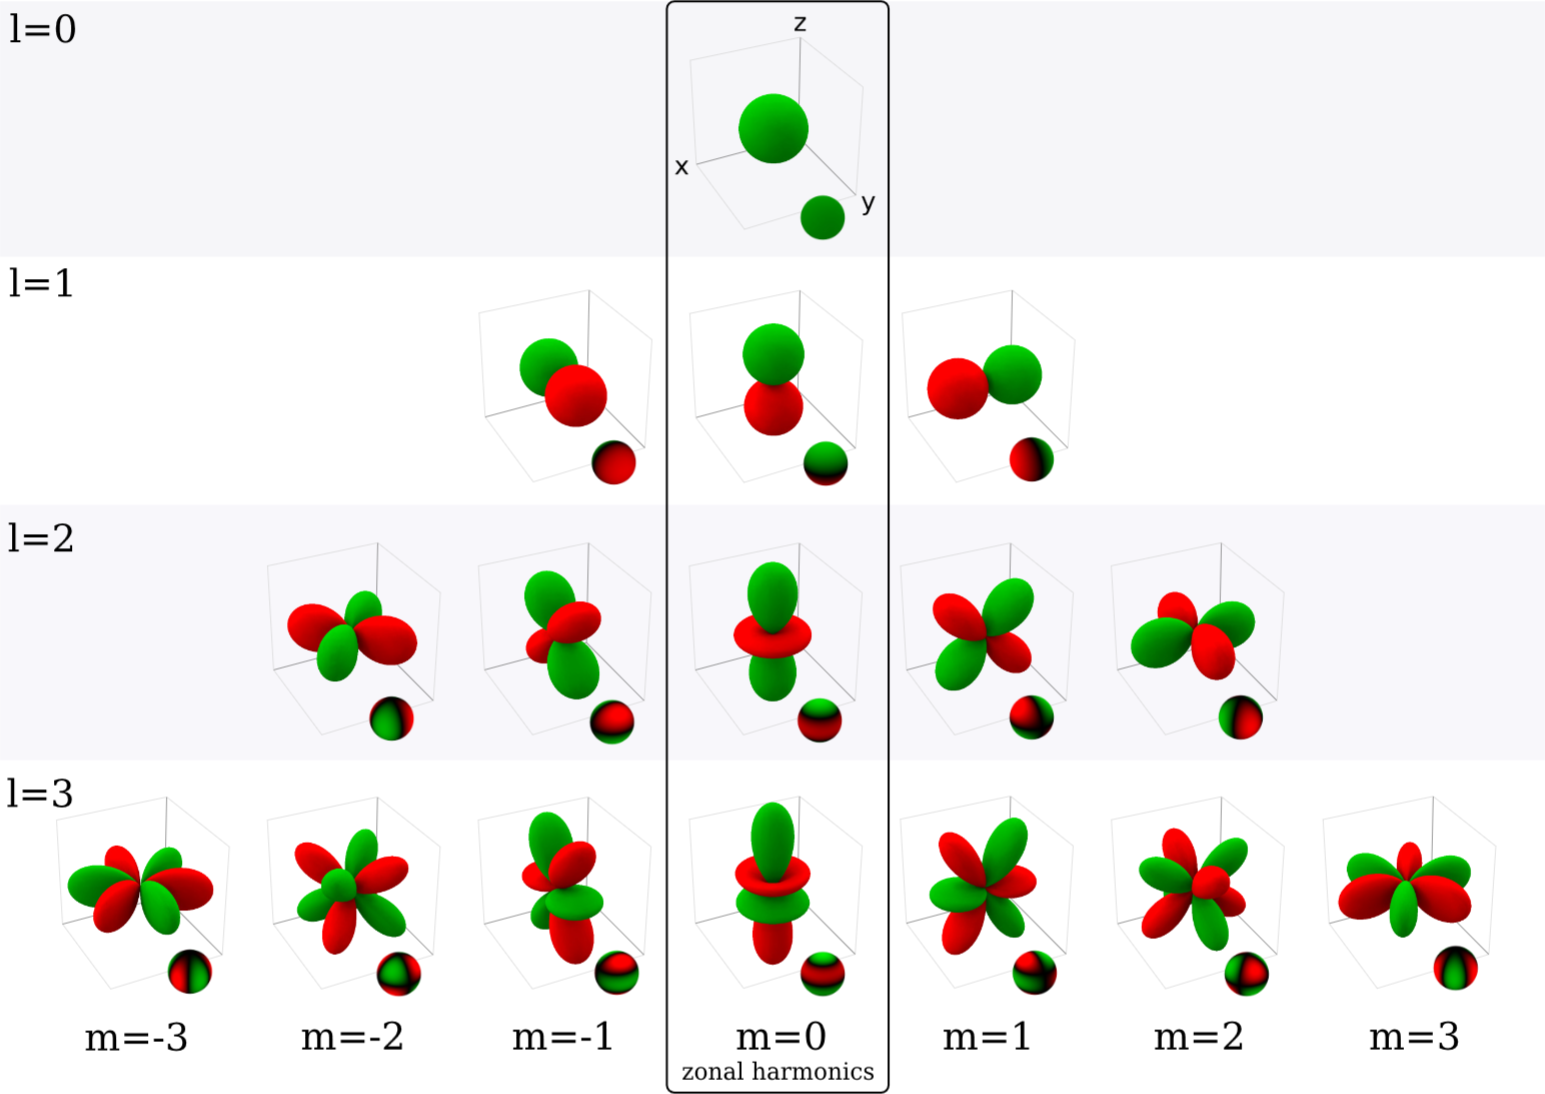
\includegraphics[width=\textwidth]{sh}
	\caption{\cite{bib:grittysph} The first three SH bands plotted as unsigned spherical functions by distance from the origin unit sphere. Green are positive values, red are negative ones.}
	\label{fig:shvisualization}
\end{figure}
\todo{Better image quality!}
The SH functions in general are defined on imaginary numbers, but for use in computer graphics usually only real-number Spherical Harmonics are relevant.

$y^m_l(\theta, \varphi)$ represents a Spherical Harmonic function.
The angles $\theta$ and $\varphi$ give a point on the unit hemisphere.
To convert from spherical to cartesian coordinates we use the following conversion:
\begin{equation} \label{equ:postoangle}
(\sin\theta\cos\varphi, \sin\theta\sin\varphi, \cos\theta) \rightarrow (x,y,z)
\end{equation}
The index $l$ represents the Spherical Harmonic \emph{band}.
Each band consists of polynomials of the degree $l$ (zero is a constant function, 1 is linear, etc.).
There are $2l+1$ functions for a given band.
Accordingly, the higher the band index $l$, the higher is the frequency of the information that is encoded in this band.
\autoref{fig:shvisualization} visualizes the first three bands.

$y^m_l(\theta, \varphi)$ is defined as:
\begin{equation}
	\begin{alignedat}{2}
		y^m_l(\theta, \varphi) &= \begin{cases}
		\sqrt{2}K^m_l \cos(m\varphi) P^m_l(\cos\theta) & m>0\\
		\sqrt{2}K^m_l \sin(-m\varphi) P^{-m}_l(\cos\theta) & m<0\\
		K^0_l P^0_l(\cos\theta) & m=0.\end{cases}
	\end{alignedat}
\end{equation}
Where $P^m_l(x)$ are the associated \emph{Legendre} polynomials and $K^m_l$ are normalization constants defined as:
\begin{equation}
	K^m_l = \sqrt{\frac{(2l+1)(l-|m|)!}{4\pi(l+|m|)!}}
\end{equation}

The associated Legendre polynomials are recursively defined as following:
\begin{equation}
	\begin{alignedat}{2}
		P^0_0(x) &= 1\\
		P^m_m(x) &= (1-2m)P^{m-1}_{m-1}\\
		P^m_{m+1}(x) &= x(2m+1)P^m_m\\	
		P^m_l(x) &= \frac{x(2l-1)P^m_{l-1}(x)-(l+m-1)P^m_{l-2}}{l-m}
	\end{alignedat}
\end{equation}


\subsection{Projection and Reconstruction} \label{chap:shprojectrecon}
Each spherical function $f(\theta, \varphi)$ can be represented with an infinite series of SH functions, each weighted by a SH coefficient.
To calculate a SH coefficient for a given band of a spherical function $f$, the product of $f$ and the SH function $y$ needs to be integrated:
\begin{equation} \label{eq:shprojection}
	c^m_l=\int\limits_{2\pi sr} f(\omega)y^m_l(\omega)\, \mathrm{d}\omega
\end{equation}
\todo{$2\pi sr$ integral must be introduced earlier}

By truncating the SH representation to $n$ bands, a function $f$ can be approximated:
\begin{equation}
	\widetilde{f}(s) = \sum_{l=0}^{n-l}\sum_{m=-l}^l c_l^m y_l^m(s)
\end{equation}

\subsection{Rotation and Zonal Harmonics} \label{sec:pre:zonalharmonics}
Spherical Harmonics are rotationally invariant:
If a function $g$ is a copy rotated by $R$ named $f$, then for the corresponding SH projections $\widetilde{g}$ and $\widetilde{f}$ it is true that:
\begin{equation}
	\widetilde{g}(s) = \widetilde{f}(R(s))
\end{equation}
This means that it is possible to rotate a function in its SH representation, without losing precision (other than rounding errors).

Later on this property will be very useful combined with \emph{Zonal Harmonics}.
Zonal Harmonics are SH projections of functions that have rotational symmetry around an axis.
If the axis is Z (in respect to \autoref{equ:postoangle}), then only the $c^m_0$ coefficients of the SH projection will be non-zero.\\
Rotation of such Zonal Harmonics $z_l$ to a new direction $d$ is generally much easier than arbitrary SH.
The resulting, rotated Spherical Harmonics coefficients are obtained as:
\begin{equation} \label{eq:zonalrotate}
	c_l^m = \sqrt{\frac{4\pi}{2l+1}} z_l y_l^m(d)
\end{equation}
\todo{Image of Zonal Harmonics}

\subfilebib % Makes bibliography available when compiling as subfile
\end{document}